\documentclass[12pt]{article}
\usepackage[margin=2.5cm]{geometry}
\usepackage{enumerate}
\usepackage{amsfonts}
\usepackage{amsmath}
\usepackage{fancyhdr}
\usepackage{amsmath}
\usepackage{amssymb}
\usepackage{amsthm}
\usepackage{mdframed}
\usepackage{graphicx}
\usepackage{subcaption}
\usepackage{adjustbox}
\usepackage{listings}
\usepackage{xcolor}
\usepackage{booktabs}
\usepackage[utf]{kotex}
\usepackage{hyperref}

\definecolor{codegreen}{rgb}{0,0.6,0}
\definecolor{codegray}{rgb}{0.5,0.5,0.5}
\definecolor{codepurple}{rgb}{0.58,0,0.82}
\definecolor{backcolour}{rgb}{0.95,0.95,0.92}

\lstdefinestyle{mystyle}{
    backgroundcolor=\color{backcolour},
    commentstyle=\color{codegreen},
    keywordstyle=\color{magenta},
    numberstyle=\tiny\color{codegray},
    stringstyle=\color{codepurple},
    basicstyle=\ttfamily\footnotesize,
    breakatwhitespace=false,
    breaklines=true,
    captionpos=b,
    keepspaces=true,
    numbers=left,
    numbersep=5pt,
    showspaces=false,
    showstringspaces=false,
    showtabs=false,
    tabsize=1
}

\lstset{style=mystyle}

\pagestyle{fancy}
\renewcommand{\headrulewidth}{0.4pt}
\lhead{CSC 209}
\rhead{Review 6 Solution}

\begin{document}
\title{CSC 209 Review 6 Solution}
\maketitle

\bigskip

\begin{enumerate}[1.]
    \item

    I need to create a wrapper function \texttt{my\_malloc} that does the following:

    \bigskip

    \begin{itemize}
        \item ask \texttt{my\_malloc} it to allocate \texttt{n} bytes
        \item call \texttt{malloc}
        \item test \texttt{malloc} doesn't have a null pointer
        \item return pointer from \texttt{malloc}
    \end{itemize}

    \bigskip

    The solution to this problem is:

\begin{lstlisting}[language=c]
    void *my_malloc(int n) {
        void *p;

        p = malloc(n);

        if (!p) {
            printf("ERROR: Malloc allocation failed");
        }

        return p;
    }
\end{lstlisting}

    \underline{\textbf{Notes}}

    \begin{itemize}
        \item Learned that void function can return value
        \item \textbf{Dynamic Storage Allocation}

        \begin{itemize}
            \item Allows to allocate storage during program execution
            \item Allows to create data structures and shink and grow array as needed
            \item e.g. \texttt{malloc}, \texttt{calloc}, \texttt{realloc}
        \end{itemize}
        \item \textbf{Memory Allocation Functions}

        \begin{itemize}
            \item \texttt{malloc} - Allocates a block of memory but doesn't initialize it

            \begin{itemize}
                \item doesn't initialize the allocated memory
                \item more efficient than \texttt{calloc}
                \item accessing the content $\to$ segmentation fault (accessing value at invalid mem. location)
                or garbage values
            \end{itemize}

            \item \texttt{calloc} - Allocates a block of memory and clears it

            \begin{itemize}
                \item allocates memory and \underline{initializes the memory block} to zero
                \item accessing the content of blocks would return 0
            \end{itemize}

            \item \texttt{realloc} - Resizes a previously allocated block of memory
        \end{itemize}

        \item \textbf{Null Pointer}

        \begin{itemize}
            \item is returned when it fails to allocate a block of memory large
            enough to satisfy the request
        \end{itemize}

        \bigskip

        \underline{\textbf{Example}}

        \begin{center}
        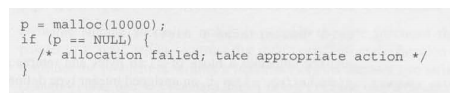
\includegraphics[width=\linewidth]{images/review_6_solution_1.png}
        \end{center}
    \end{itemize}

    \item

    I need to write a function named \texttt{duplicate} that uses dynamic storage
    allocation to create a copy of a string.

    \bigskip

    The requirements of the function are

    \begin{itemize}
        \item \texttt{duplicate} allocates space for a string of the same length as \texttt{str}
        \item \texttt{duplicate} copies the contents of str into the new string
        \item \texttt{duplicate} returns a pointer to it
        \item \texttt{duplicate} returns a null pointer if the memory allocation fails
    \end{itemize}

    \bigskip

    The solution to this problem is included in file \texttt{question\_2.c}

    \bigskip

    \underline{\textbf{Note}}

    \begin{itemize}
        \item \texttt{const} tag in parameter prevetns the function from modifying
        what it's pointer variable is pointing to.

        \begin{itemize}
            \item value is modifiable
            \item changes the parameter to pass by value
        \end{itemize}
    \end{itemize}
\end{enumerate}

\end{document}